% !TeX spellcheck = en-US
% !TeX encoding = utf8
% !TeX program = pdflatex
% !BIB program = biber
% -*- coding:utf-8 mod:LaTeX -*-


% vv  scroll down to line 200 for content  vv


\let\ifdeutsch\iffalse
\let\ifenglish\iftrue


\input{pre-documentclass}
\documentclass[
  %
  %ngerman, %%% Add if you write in German.
  %
  % fontsize=11pt is the standard
  a4paper,  % Standard format - only KOMAScript uses paper=a4 - https://tex.stackexchange.com/a/61044/9075
  twoside,  % we are optimizing for both screen and two-side printing. So the page numbers will jump, but the content is configured to stay in the middle (by using the geometry package)
  bibliography=totoc,
  %               idxtotoc,   %Index ins Inhaltsverzeichnis
  %               liststotoc, %List of X ins Inhaltsverzeichnis, mit liststotocnumbered werden die Abbildungsverzeichnisse nummeriert
  headsepline,
  cleardoublepage=empty,
  parskip=half,
  %               draft    % um zu sehen, wo noch nachgebessert werden muss - wichtig, da Bindungskorrektur mit drin
  draft=false
]{scrbook}
\input{config}


\usepackage[
  title={Alerting Users to Phishing Threats: A Comprehensive Evaluation of Warning Techniques}, % Do not forget to capitalize your title correctly, you may use the following page to help you: https://capitalizemytitle.com/
  author={Yunus Emre Yavuz},
  orcid=0009-0009-6762-8269, % get your own ORCID via https://orcid.org/
  email={yunus.yavuz@campus.lmu.de},
  type=bachelor,
  institute={Institut für Informatik}, % or other institute names - or just a plain string using {Demo\\Demo...}
  examiner={Univ.-Prof.\ Dr.\ Florian Alt},
  supervisor={Dr.\ Verena Distler,\\Felix Dietz,\ M.Sc.},
  startdate={20.01.2024},
  enddate={01.07.2024},
  % Falls keine Lizenz gewünscht wird bitte auf "none" setzen
  % Die Lizenz erlaubt es zu nichtkommerziellen Zwecken die Arbeit zu
  % vervielfältigen und Kopien zu machen. Dabei muss aber immer der Autor
  % angegeben werden. Eine kommerzielle Verwertung ist für den Autor
  % weiter möglich.
  copyright=ccbysa, % ccbysa, ccbynosa, cc0, none
  language=english
]{lmu-thesis-cover}

\usepackage{tabularx}
\usepackage{caption}
\usepackage{subcaption}
\usepackage{tikz-uml}
\usepackage{float}
\usepackage{pgfplots}
\usepackage{booktabs}
\usepackage{color}
\usepackage{tabularray}
\usepackage{wrapfig}
\usepackage{fontawesome} 
\usepgfplotslibrary{statistics}
\pgfplotsset{width=10cm,compat=1.15}
% Hier stehen alle Abkürzungen
\newacronym{aoi}{AOI}{Area of Interest}
\newacronym{qda}{QDA}{Qualitative Data Analysis}
\newacronym{ati-s}{ATI-S}{Affinity for Technology Interaction Short Scale}


\makeindex


\begin{document}

%tex4ht-Konvertierung verschönern
\iftex4ht
  % tell tex4ht to create picures also for formulas starting with '$'
  % WARNING: a tex4ht run now takes forever!
  \Configure{}{\PicMath}{\EndPicMath}{}
  %$ % <- syntax highlighting fix for emacs
  \Css{body {text-align:justify;}}

  %conversion of .pdf to .png
  \Configure{graphics*}
  {pdf}
  {\Needs{"convert \csname Gin@base\endcsname.pdf
      \csname Gin@base\endcsname.png"}%
    \Picture[pict]{\csname Gin@base\endcsname.png}%
  }
\fi

%\VerbatimFootnotes %verbatim text in Fußnoten erlauben. Geht normalerweise nicht.

\input{commands}
\pagenumbering{arabic}
\Coverpage
\Copyright
%Eigener Seitenstil fuer die Kurzfassung und das Inhaltsverzeichnis
\deftriplepagestyle{preamble}{}{}{}{}{}{\pagemark}
%Doku zu deftriplepagestyle: scrguide.pdf
\pagestyle{preamble}
\renewcommand*{\chapterpagestyle}{preamble}



%Kurzfassung / abstract
%auch im Stil vom Inhaltsverzeichnis
\section*{Kurzfassung}
Phishing-Angriffe sind trotz diverser Fortschritte im Bereich der Cybersicherheit nach wie vor eine große Bedrohung. Diese Arbeit befasst sich mit der Verbesserung der Erkennung und Reaktion auf Phishing durch die Gestaltung und Implementierung visueller Warnungen in E-Mail-Clients. Über einen Zeitraum von zwei Wochen wurde eine Mixed-Methods-Studie mit 16 Teilnehmern durchgeführt, in der Eye-Tracking-Technologie und qualitatives Feedback integriert wurden, um die Interaktionen mit verschiedenen Phishing-Warnungen in Mozilla Thunderbird zu bewerten. \newline
Eye-Tracking-Daten zeigten, dass unmittelbare und prominent platzierte Warnungen effektiver sind, während periphere Warnungen tendenziell erst später wahrgenommen werden, was ihre Effektivität in realen Szenarien verringern könnte. Qualitatives Feedback unterstrich die Bedeutung von Klarheit, Kontext und lehrreichen Inhalten in den Warnhinweisen, um das Verständnis der Benutzer zu verbessern und Phishing-Angriffe zu verhindern. \newline
Diese Ergebnisse legen nahe, dass die Gestaltung von Phishing-Warnungen erhebliche Auswirkungen auf die Cybersicherheit haben kann. Durch die Konzentration auf benutzerzentrierte Warnhinweise, die sowohl auffällig als auch informativ sind, können die Abwehrmechanismen von Phishing-Angriffen erheblich gestärkt werden. Diese Forschungsarbeit leistet einen Beitrag zum breiteren Feld der Cybersicherheit, indem sie evidenzbasierte Empfehlungen für die Gestaltung effektiver Phishing-Warnungen liefert, die darauf abzielen, die Prävalenz und die Auswirkungen von Phishing zu reduzieren. 

\cleardoublepage

\section*{Abstract} 
Phishing attacks remain a significant threat despite advancements in cybersecurity. This thesis addresses the enhancing of user detection and response to phishing through the design and implementation of visual warnings within email clients. Over a two-week period, a mixed-methods study involving 16 participants was conducted, integrating eye tracking technology and qualitative feedback to assess interactions with various phishing warning designs in Mozilla Thunderbird. \newline
Eye tracking data revealed that immediate and prominently placed warnings are more effective, while peripheral warnings tend to be noticed later, potentially reducing their effectiveness in real-world scenarios. Qualitative feedback highlighted the importance of clarity, context, and educational content in warnings to enhance user understanding and prevent phishing attacks. \newline
These findings suggest that the design of phishing warnings can have substantial implications for cybersecurity. By focusing on user-centric warning designs that are both noticeable and informative, phishing defense mechanisms can be significantly strengthened. This research contributes to the broader cybersecurity field by providing evidence-based recommendations for designing effective phishing warnings, aiming to reduce the prevalence and impact of phishing attacks across digital platforms.

\cleardoublepage


% BEGIN: Verzeichnisse

\iftex4ht
\else
  \microtypesetup{protrusion=false}
\fi

%%%
% Literaturverzeichnis ins TOC mit aufnehmen, aber nur wenn nichts anderes mehr hilft!
% \addcontentsline{toc}{chapter}{Literaturverzeichnis}
%
% oder zB
%\addcontentsline{toc}{section}{Abkürzungsverzeichnis}
%
%%%

%Produce table of contents
%
%In case you have trouble with headings reaching into the page numbers, enable the following three lines.
%Hint by http://golatex.de/inhaltsverzeichnis-schreibt-ueber-rand-t3106.html
%
%\makeatletter
%\renewcommand{\@pnumwidth}{2em}
%\makeatother
%
\tableofcontents

% Bei einem ungünstigen Seitenumbruch im Inhaltsverzeichnis, kann dieser mit
% \addtocontents{toc}{\protect\newpage}
% an der passenden Stelle im Fließtext erzwungen werden.

\listoffigures
\listoftables


% Control List of Listings
\let\iflistings\iffalse
%Wird nur bei Verwendung von der lstlisting-Umgebung mit dem "caption"-Parameter benoetigt
%\lstlistoflistings
%ansonsten:
\iflistings
  \ifdeutsch
    \listof{Listing}{Verzeichnis der Listings}
  \else
    \listof{Listing}{List of Listings}
  \fi
\fi

% Control List of Algorithms
\let\ifalgorithms\iffalse
\ifalgorithms
  %mittels \newfloat wurde die Algorithmus-Gleitumgebung definiert.
  %Mit folgendem Befehl werden alle floats dieses Typs ausgegeben
  \ifdeutsch
    \listof{Algorithmus}{Verzeichnis der Algorithmen}
  \else
    \listof{Algorithmus}{List of Algorithms}
  \fi
  %\listofalgorithms %Ist nur für Algorithmen, die mittels \begin{algorithm} umschlossen werden, nötig
\fi

% Control Glossary
\let\ifglossary\iffalse
\ifglossary
  \printnoidxglossaries
\fi

\iftex4ht
\else
  %Optischen Randausgleich und Grauwertkorrektur wieder aktivieren
  \microtypesetup{protrusion=true}
\fi

% END: Verzeichnisse


% Headline and footline
\renewcommand*{\chapterpagestyle}{scrplain}
\pagestyle{scrheadings}
\pagestyle{scrheadings}
\ihead[]{}
\chead[]{}
\ohead[]{\headmark}
\cfoot[]{}
\ofoot[\usekomafont{pagenumber}\thepage]{\usekomafont{pagenumber}\thepage}
\ifoot[]{}

%%%%%%%%%%%%%%%%%%%%%%%%%%%%%%%%%%%%%%%%%%%%%%%%%%%%%%%%%%%%%%%%%%%%%%%%%%%%%%
%
% Main content starts here
%
%%%%%%%%%%%%%%%%%%%%%%%%%%%%%%%%%%%%%%%%%%%%%%%%%%%%%%%%%%%%%%%%%%%%%%%%%%%%%%


\chapter{Introduction}
\label{sec:introduction}
In today's digital age, the internet is integral to daily activities such as communication, transactions, and accessing information. Yet, this increased dependency brings heightened security risks, especially from phishing attacks. Phishing, a prevalent cyber threat, involves deceiving individuals into revealing sensitive information by masquerading as a trustworthy entity in digital communications. There is a vast amount of phishing vectors, such as SMS, social media or email, with the latter being the most common medium for phishing attacks \cite{verizon}. These attacks are used to direct victims to fraudulent websites where they are coerced into providing personal and financial details, allowing attackers unauthorized access to accounts \cite{Wang2012}. \newline 
The impact of phishing extends beyond individual victims to organizations worldwide, causing significant financial losses and eroding trust in digital systems. In 2023, the Anti-Phishing Working Group (AWPG) observed approximately 4.9 Million phishing attacks \cite{apwg}. Despite the deployment of various anti-phishing technologies, the human factor remains a critical vulnerability. The effectiveness of phishing warnings, therefore, is paramount in the cybersecurity defense arsenal. These warnings, if designed and implemented effectively, can play a crucial role in educating users and averting the success of phishing attacks. \par
In response to the escalating threat of phishing attacks, numerous efforts have been undertaken by cybersecurity experts and organizations to mitigate the risks. These include the development of algorithms for threat detection \cite{thakur} and the implementation of user awareness programs \cite{jampen}. Users' ability to detect and respond to phishing attempts is critical, prompting a shift toward developing more user-centered security solutions. These solutions emphasize visual warnings that act as direct interventions, alerting users to potential threats. However, the effectiveness of such warnings hinges on several factors that this study aims to explore and understand. \par
For our study, we developed mock-up visual warnings to simulate real alerts in an email client and expanded their functionality with a custom plugin for Mozilla Thunderbird, a widely-used open-source email client chosen for its adaptability. This plugin enhances the visual presentation of phishing warnings, utilizing common design principles to capture users' attention more effectively. \newline
We created a unique set of emails incorporating both regular communications and mock phishing scenarios to simulate a realistic email environment. Using eye tracking technology and detailed user feedback, we explored how users perceive, understand, and react to various visual warning strategies. This investigation offers insights into the design of more effective phishing warnings and highlights the importance of user interface design in cybersecurity. By focusing on user-centric design elements, our study aims to improve how visual cues are used to strengthen defenses against phishing attacks. Our research is structured around the following research questions:

\begin{itemize}
    \item RQ1: How do users' perceptions differ in response to various phishing warnings in email interfaces, and which type is perceived as the most effective? \textit{Here, "effective" refers to the ability of the warnings to increase user awareness, prompt appropriate user actions to mitigate risk (e.g., not clicking on malicious links), and enhance recognition of phishing threats in future encounters.}
        \begin{itemize}
            \item How do users perceive the helpfulness of each warning type?
        \end{itemize}
        \begin{itemize}
            \item Which warning design do users prefer and why?
        \end{itemize}
    \item RQ2: What common gaze patterns emerge among users when scanning email content, and how can these patterns help with the strategic placement of phishing warnings to maximize user attention?
\end{itemize}

To adress these research question we have laid out the following objectives for our study:

\begin{enumerate}
    \item \textit{Evaluating Visual Warning Strategies:} We aim to examine the effectiveness of various visual elements (e.g. banner placement, animations) in warning designs in terms of their immediate recognizability and understandability.
    \item \textit{Analyzing Attention Distribution:} Using eye tracking technology, we plan to identify which visual elements attract users' attention and how these elements influence perception and behaviour.
    \item \textit{Assessing User Reactions:} Through interviews with participants, we intend to capture their subjective evaluations and opinions regarding the different warning types. This includes exploring user trust and their perception on the warnings helpfulness.
    \item \textit{Establishing Best Practices:} Based on the collected data and user feedback, we seek to identify design principles that maximize the effectiveness of phishing warnings.
\end{enumerate}

In summary, our research reveals that effectively designed phishing warnings can significantly influence users' abilities to recognize and respond to phishing attempts. Eye tracking data confirmed that warnings integrated within the email body are noticed and acted upon more swiftly than those placed peripherally or appearing with a delay. Qualitative feedback underscored the importance of clear, contextual information within these warnings, enhancing users' understanding of potential threats. \newline
The implications of these results are substantial, advocating for a shift in how cybersecurity defenses are structured. As phishing tactics evolve, the need for warnings that seamlessly integrate into users' workflows and effectively communicate risks becomes increasingly critical. By focusing on the development of user friendly and informative warning systems, we can better equip individuals to combat phishing threats, potentially reducing the success rate of such attacks across various platforms. 

%LaTeX hints are provided in \autoref{chap:latexhints}.

\chapter{Background and Related Work}
\label{sec:relatedwork}

In the dynamic field of cybersecurity, understanding the multifaceted nature of phishing attacks is essential for developing effective defensive strategies. This section provides an overview of the key areas of research that inform our study on phishing warnings. By exploring the psychological underpinnings of social engineering, the evolution of phishing detection technologies, and the critical role of user education, we aim to contextualize our research within the broader discourse on combating phishing. Each of these areas offers vital insights that directly influence the design and implementation of phishing warnings, ensuring they are not only technically sound but also psychologically effective.

\section{Phishing Definition and Techniques}
Phishing is a deceptive practice where cybercriminals use fraudulent communication, typically via email, to trick individuals into revealing personal information, such as passwords and credit card numbers. This cyber threat exploits the trust of users through cleverly disguised messages that mimic legitimate sources. Understanding the array of phishing techniques is essential for developing effective countermeasures and for training users to recognize and avoid these threats.

As detailed by Alkhalil et al. \cite{alkhalil}, phishing attacks employ a combination of technical and psychological tactics to extract sensitive information from victims. These attacks are not uniform but vary significantly in their approach and execution.
Alkhalil et al. identify several prevalent phishing techniques:
\begin{itemize}
    \item \textit{Email Phishing:} The primary method where attackers send fraudulent emails mimicking legitimate sources to steal personal information. Visual warnings for this technique should clearly differentiate genuine communications from phishing attempts, for instance by highlighting suspicious elements directly within the email interface.
    \item \textit{Spear Phishing and Whaling:} Highly targeted forms that use personalized information to increase the attack's credibility.
    \item \textit{Vishing (Voice Phishing) and SMiShing (SMS Phishing):} Phishing via phone calls and SMS that exploit the user's trust in mobile communications.
    \item \textit{Website Forgery:} Creating counterfeit websites that replicate genuine ones to capture personal data.
    \item \textit{Social Media Phishing:} Using social platforms to trick users into revealing sensitive data through deceptive posts or messages.
\end{itemize}

This classification underscores the importance of tailored defensive strategies that address the specific vectors and tactics of each phishing type, enhancing both technological defenses and user training programs.

\section{Technical Detection Strategies}
Phishing detection technologies are essential tools, designed to identify and mitigate phishing attempts across various digital platforms. Among these technologies, email client spam filters, with phishing emails being a subset of spam mails, represent a fundamental line of defense, filtering out potential phishing emails based on specific criteria such as sender reputation \cite{shi} or message content \cite{alexy}.

In their paper, Bhomwick et al. \cite{alexy} delve into the evolution of machine learning techniques in the realm of email spam filtering. They chart the journey from initial heuristic-based approaches to the adoption of sophisticated machine learning models, capable of dynamically adapting to the continually evolving strategies employed by spammers. The paper not only highlights the effectiveness of these techniques but also points towards future directions for research in improving spam detection mechanisms.

Another approach in phishing detection is explored by Md. Abu Ashraf Siddiq et al. \cite{siddiq}, utilizing deep learning techniques. Their study, employing neural networks, showcases the potential of deep learning in accurately identifying phishing websites. This highlights deep learning's pivotal role in cybersecurity, especially in distinguishing malicious content, and emphasizes its contribution to advancing phishing detection systems.

While technological solutions are crucial, their effectiveness ultimately depends on the users' ability to understand and respond to the warnings they generate. This interdependency brings our research into focus, aiming to optimize visual warnings to ensure they not only capture attention but also convey urgency effectively, prompting appropriate user actions in the face of potential threats.

\section{User Education and Training}
Understanding the mechanisms behind phishing attacks and the reasons users fall prey to them is essential in developing effective countermeasures. A key vulnerability is the general lack of cybersecurity awareness among users, rendering them susceptible to manipulation by attackers. In their paper Dhamija et al. \cite{dhamija} highlight this issue, pointing out the critical need for enhanced user understanding to mitigate vulnerability to phishing shemes. 

To adress this gap, various training methods have been explored, aiming to improve user ability to recognize and resist phishing attempts. Research by Sheng et al. \cite{sheng} showcases an innovative approach in phishing education through the 'Anti-Phishing Phil' game. This research demonstrates that integrating educational content with interactive gameplay can significantly increase the efficacy of cybersecurity training. Such engaging methods not only educate but also actively involve users in the learning process, making the lessons more memorable and practical. 

Further emphasizing the importance of user education, Kumaguru et al. \cite{kumaraguru} investigated the impact of training on users' abilites to distinguish between legitimate and fraudulent websites. Their findings underscore the effectiveness of well-crafted educational programs in empowering users against phishing threats. 

Additionally, Wash's article \cite{wash} on how IT experts detect phishing emails provides a unique perspective on the cognitive strategies employed by experienced professionals. By interviewing IT experts, Wash explains a three-stage process these professionals use: sensemaking, suspicion, and decision-making, when evaluating the legitimacy of an email. This approach underscores the depth of expertise and vigilance required to effectively identify phishing attempts, highlighting the potential benefits of training programs.

Integrating these insights, our study leverages the principles of effective education and cognitive engagement in designing visual warnings that are not only noticeable but also informative. By enhancing user understanding of what phishing attempts look like, we aim to elevate the baseline of cybersecurity awareness.

\section{Social Engineering in Phishing}
Social engineering is described as an attack type where the assailant exploits human vulnerabilities through social interaction to compromise cybersecurity goals like confidentiality, integrity, and availability of cyber elements. Unlike traditional attacks that may require overcoming technical barriers, social engineering attacks manipulate human psychology to bypass security measures. It's particularly challenging to defend against because it preys on innate human traits, which can often be turned into security vulnerabilities by skilled attackers \cite{Wang2021}.

%Exploring vulnerability in social networks, Albladi et al. \cite{albladi} analyze factors that predict individuals' vulnerability to social engineering in social networks. It proposes a model incorporating user characteristics such as level of involvement, social network experience, and perceptual factors like risk perception and competence. This research aims to identify the most vulnerable users for targeted training programs, contributing to safer social networking practices.

Highlighting persuasive email techniques, Koddebusch \cite{koddebusch} focuses on the specific persuasive techniques employed in phishing emails, such as invoking authority or urgency, which effectively manipulate users' decision-making processes. This manipulation illustrates how cyber attackers exploit psychological triggers to induce actions that users might otherwise consider risky or unnecessary. Koddebusch's findings provide empirical evidence that these persuasion strategies significantly increase the success rate of phishing attacks, underscoring the critical need for awareness and training that can help individuals recognize and resist such tactics. 

In their research, Abdrabou et al. \cite{abdrabou} investigate how phishing emails affect user behavior by tracking their gaze and mouse movements during an email sorting task. The study aims to understand if these physiological and behavioral cues can serve as indicators of exposure to phishing attacks, which are often designed to manipulate users into revealing sensitive information. Their findings suggest that subtle changes in behavior, such as eye movements or mouse dynamics, could potentially be used to identify when users are interacting with phishing content. 

Distler's study \cite{distler} examines the impact of various contextual factors on individuals' responses to phishing within an organizational setting. Using an in-situ deception methodology with 14 participants in their real work environments, the study reveals that contexts significantly influence the likelihood of falling for phishing emails. Distler's findings underscore the importance of contextualized training and proactive organizational policies to enhance cybersecurity. The research also underscores the role of language and writing style in the detection of phishing mails, revealing that unexpected variations in these elements can alert recipients to potential phishing attempts. 

Building on these findings, our study introduces and evaluates targeted phishing warnings that focus on anomalies in greeting patterns and email signatures—common areas where deviations from normative language use might occur. By flagging unusual language patterns that recipients have learned to associate with phishing these warnings aim to enhance the detection capabilities of email users, potentially increasing their vigilance and reducing the likelihood of successful phishing attacks. 

\chapter{Methodology}
\label{sec:methodology}
\section{Research Design}
Our study adopts a mixed-methods approach, integrating eye tracking data and qualitative interviews to examine how users perceive and interact with phishing warnings in email interfaces. The quantitative component makes use of eye tracking to objectively measure user attention and gaze patterns across various warning designs. The qualitative segment, through semi-structured interviews, investigates participant perspectives, enriching the data with personal insights and preferences. This dual-faceted approach aims to reveal not only immediate visual engagements but also deeper user experiences.

\section{Research Setting}
Our research was conducted in a controlled lab environment at the University of the Bundeswehr. Upon arrival, participants were welcomed and escorted to a dedicated workstation, which was arranged to facilitate the study's requirements. This workstation was equipped with a computer system that had the email client, Mozilla Thunderbird, preloaded and configured for immediate use. An eye tracking device was connected to the computer to record and analyze participants' gaze patterns as they interacted with the email client. The setting was optimized to mimic a typical user experience while ensuring precise data capture for the study's analysis.

\section{Recruitment of Participants}
For the recruitment of participants for this study, we utilized multiple communication channels within the informatics community of the University. The study was advertised in group chats on popular platforms such as Discord, Whatsapp and Slack. Additionally, we utilized the LMU newsletter to reach a broader audience within the university setting. There were no specific prerequisites for participants, allowing for a wide demographic range. The study was open to all indiviuals aged 18 and above. Participants received a 10 EUR compensation for their participation.

\section{Material}
\subsection{Technical Equipment and Tools}
Central to this study is the integration of eye tracking technology, specifically utilizing the Tobii Pro Spark eye tracker in conjunction with the Tobii Pro Lab software. This setup plays a crucial role in objectively capturing where participants' attention is focused as they interact with email content and phishing warnings. By recording gaze patterns we gain valuable insights into the reactions to different warning designs. The Tobii Pro Lab software allows us the seamless recording of the participants' screen alongside their gaze movements and patterns, simplifying a comprehensive analysis of the captured data. \newline 
Audio recording was conducted using a Google Pixel smartphone, which features built-in auto transcription software, providing us with a reliable method for capturing and transcribing participant feedback during the study. Each transcript was additionally manually reviewed to ensure the accuracy of the data and to filter out irrelevant or personal information.

\subsection{Emails}
To establish a genuine email environment for the study, we created a suite of 30 emails to mirror the typical inbox of a professional workspace. This collection included routine business correspondences, such as project updates, meeting invitations, and newsletters, mixed with 9 simulated phishing emails. The inclusion of one false negative, a phishing email not recognized as such, further emulates the realistic challenges users face. These simulations employed prevalent phishing strategies observed in actual attacks, such as soliciting confidential information, fraudulent alerts, and deceptive links to malicious websites.

\begin{figure} [ht]
    \centering
    \includegraphics[width=0.8\linewidth]{figures/example2.png}
    \caption{Participants' environment in Mozilla Thunderbird.}
    \label{fig:example2}
\end{figure}

\begin{figure} [ht]
    \centering
    \includegraphics[width=0.6\linewidth]{figures/example.png}
    \caption{An example for a mock phishing email.}
    \label{fig:example}
\end{figure}

\section{Procedure}

\subsection{Consent, Demographics and ATI-S}

Before beginning with the study tasks, participants are required to sign a consent form that includes permissions for screen and audio recording as well as eye tracking. Following consent, they are asked to provide demographic information such as age, gender, educational background, and professional experience. Additionally, participants fill out the short version of the Affinity for Technology Interaction Scale (ATI-S)\footnote{https://ati-scale.org/}. This scale assesses individuals' comfort levels and predispositions towards technology, which helps to illuminate how these factors may influence their perceptions and interactions with phishing warnings. \newline
We opted to use the short version of the ATI scale due to its ability to efficiently measure technological affinity without imposing extensive questionnaire fatigue on participants and maintaining high engagement levels.

\subsection{Briefing and Setup}

Participants receive a briefing on the eye tracking process and a brief overview of Mozilla Thunderbird if they are not already familiar with its interface. The eye tracking calibration is conducted next to ensure accurate data capture. Audio recording is also enabled to capture the participants' verbal feedback throughout the study, facilitating later analysis of their qualitative responses. Participants are informed that they are welcome to ask questions at any time during the study to clarify any doubts or concerns they may have.

\subsection{Phase One: Sorting Task and Collection of Eyetracking Data}

Phase One serves as the quantitative backbone of our study, utilizing eye tracking technology to gather gaze data as participants engage with a series of emails. This phase is designed to simulate a real-world working environment to objectively assess how participants interact with our phishing warnings in a typical workflow. 

\textbf{Task Setup and Environment}

Participants are cast in the role of an employee at the fictional company "CloudTech". This setup is intended to create a realistic email environment. Upon commencement they are provided with a folder containing a mix of emails, including routine communications from fictional colleagues and company announcements. Within these emails there are several phishing attempts, though participants are not made aware of these inclusions to avoid biasing their responses.  

\textbf{Instructions and Procedure}

To simplify the email management task and ensure clarity, participants are instructed to discard any email into the trash folder that they suspect or deem unnecessary, without the need to further categorize or mark emails. This is designed to streamline the sorting process, allowing participants to focus more on the content and less on organizational tasks. 
During the sorting process, participants are encouraged to verbalize their thoughts and decisions. This "think aloud" method is crucial for understanding the decision-making process behind their actions.
\newpage
\textbf{Observer Role and Time Allocation}

The observer's role during this phase is to listen and monitor the explanations provided by the participants, intervening minimally (e.g. when questions arise) to avoid influencing their natural behavior. Each participant is allocated approximately 10 minutes to complete the task.

\subsection{Phase Two: Gathering Qualitative Feedback}

Following the sorting task, participants undergo a detailed semi-structured interview. They are asked about their subjective perceptions, their strategies for identifying phishing attempts and their opinions on the clarity and effectiveness of different warning designs.
This qualitative data enriches the study’s findings by adding personal personal context to the observed behaviours and eye tracking metrics. The interview questions cover several key areas:

\begin{itemize}
    \item General Perception: Inquiry into how participants perceived the warnings overall, including any elements that particularly stood out to them and the influence of the warnings on their decision making process.
    \item Effectiveness: Evaluation of the warnings' effectiveness presented during the study, identifying any warnings perceived as particularly helpful or less so. This includes a comparision between the different warnings.
    \item Design: Assessement of the warnings' design aspects, such as color, placement, and animations, and their impact on the users' attention.
    \item Personal Behaviour: Discussion around any new information noticed in the warnings that hadn't been considered before and typical behaviours when encountering phishing emails.
    \item Feedback: Suggestions for improving future iterations of the study and an opportunity for participants to raise any further questions or comments. 
\end{itemize}
 
The full study protocol and questioning framework is provided in appendix \ref{sec:protocol} and \ref{sec:interview}.

\begin{figure} [ht]
    \centering
    \includegraphics[width=1\linewidth]{figures/studysteps.png}
    \caption{Summary of the study procedure.}
    \label{fig:steps}
\end{figure}

\section{Data Analysis}
\subsection{Qualitative Data Analysis}
To enhance our understanding of participants' perceptions regarding different phishing warning designs, we employed a Qualitative Data Analysis (QDA) approach. Following established methodologies outlined in literature \cite{qda}, our method involved a hybrid coding strategy, combining both deductive and inductive techniques. Initially we established a set of codes based on our research questions and theoretical framework (deductive). As we analyzed the data, we expanded and refined this set to include new themes and patterns that emerged from participant feedback (inductive). This approach ensured that our analysis remained both structured and adaptive to the insights yielded by the study.

To ease up the exploration of qualitative data, we utilized MAXQDA2024. This software provided robust tools for organizing, coding, and analyzing the interview data, making the complex process of qualitative analysis more manageable and systematic. The project files are available in our GitHub repository, linked in appendix \ref{sec:github}.

Our coding framework captures the key dimensions of our research. Each main category and sub-category focuses on different aspects of how users interact with and perceive the visual and functional elements of phishing warnings. A detailed list of codes with explanations is provided in appendix \ref{sec:qda}. 

\begin{figure} [ht]
    \centering
    \includegraphics[width=0.9\linewidth]{figures/coding.png}
    \caption{Graphic illustration of our QDA codes, generated in MAXQDA 2024.}
    \label{fig:qda}
\end{figure}

\subsection{Eyetracking Data Analysis}
To evaluate the eye tracking data, we formulated the following hypotheses:

\begin{itemize}
    \item[\textbf{H1}] Delayed slide-in animations of warnings will disrupt typical email reading patterns and draw more attention.
    \item[\textbf{H2}] Warnings placed on the side of the email interface will be noticed later compared to those within the email body or at the top.
    \item[\textbf{H3}] Content integrated directly into the email body (e.g. Greeting or Signature Warning) will hold user attention for longer periods.
\end{itemize}

To analyze the eye tracking data, we used the Tobii Pro Lab software, which provided many tools for visualizing and interpreting gaze patterns. Our analysis involved several key tasks:

\begin{enumerate}
    \item \textbf{Defining Areas of Interest (AOI):} We defined specific AOIs within the email interface. This allowed us to quantify metrics such as fixation durations and frequencies for specific areas. The AOIs included different parts of the email where warnings were placed (see figure \ref{fig:aoi}).
    \item \textbf{Establishing Times of Interest (TOI):} To focus on critical moments of interaction, we defined TOIs. These were specific instances when participants opened emails containing warnings.
    \item \textbf{Visualization and Gaze Path Analysis:} Using Tobii Pro Lab’s visualization tools, we oberserved and analyzed gaze points. This was crucial for Hypothesis 1, as it allowed us to see how animations affected reading patterns.
\end{enumerate}

To align with our hypotheses, we collected the following eye tracking metrics:

\begin{enumerate}
    \item \textbf{Time to First Fixation:} This metric measures the time it takes for participants to fixate on a specific AOI after the email is presented \cite{eyetrack}. It helps us understand how quickly each warning design draws attention compared to others.
    \item \textbf{Average Fixation Duration:} By averaging the duration of all fixations within each AOI, we can assess the overall engagement level with different components of the email interface. Fixation durations range from 150-300ms, with higher durations meaning a higher level of engagement \cite{eyetrack}.
\end{enumerate}

These methods and metrics allowed us to test our hypotheses and evaluate the effectiveness of different phishing warning designs in capturing user attention.

\begin{figure} [ht]
    \centering
    \includegraphics[width=0.7\linewidth]{figures/aoi.png}
    \caption{AOI zones in Tobii Pro Lab.}
    \label{fig:aoi}
\end{figure}

\chapter{Design and Implementation}
\label{implementation}

\section{Warning Types}
\label{types}
For our study we designed four primary types of phishing warnings, each having two different variations. These variations aim to explore different aspects of user interaction and attention.

\subsection{Group 1: General Alerts}

\textbf{Generic Banner:} A broad, non-specific warning that does not target any specific content within the email but serves as a general alert to the possibility of phishing.

\begin{itemize}
    \item Variant 1: The banner slides in from the top. This placement tests the immediate visibility and impact of warnings when users first open an email. 
    \item Variant 2: The banner is positioned on the right side of the email body. This alternative aims to assess how peripheral placement affects user noticeability and response compared to more traditional top placement.\par
\end{itemize}

\begin{figure} [h]
\centering
\begin{subfigure}{.5\textwidth}
  \centering
  \includegraphics[width=.9\linewidth]{figures/banner1.png}
  \caption{Variant 1}
  \label{fig:banner1}
\end{subfigure}%
\begin{subfigure}{.5\textwidth}
  \centering
  \includegraphics[width=.9\linewidth]{figures/banner2.png}
  \caption{Variant 2}
  \label{fig:banner2}
\end{subfigure}
\caption{Generic Banner}
\label{fig:banner}
\end{figure}
\newpage

\subsection{Group 2: Context-Aware Warnings}

\textbf{Tooltip Warning on Link Hover:} This warning appears when a user hovers over a link, providing immediate contextual information about the potential danger of the link, making it context-aware as it is specifically related to the actions the user is about to take (i.e., clicking a link). A tooltip appears, warning the user and preventing them from clicking the link. After a 3 second countdown, the tooltip moves to the side, making the link clickable at the users own risk. 

This approach aligns closely with the research conducted by Petelka et al. \cite{petelka}, which emphasizes the effectiveness of proximity and user interaction with link-focused phishing warnings in reducing susceptibility to phishing attacks. In this thesis, the tooltip warning activates when a user hovers over a link, immediately providing contextual information and temporarily blocking access to the link, thereby forcing the user to recognize and process the warning before proceeding. This method mirrors Petelka et al.'s findings that such forced interaction can significantly heighten user caution and awareness. Our study further explores the impact of varying levels of informational detail in the tooltips, assessing how these variations influence user perception.

\begin{itemize}
    \item Variant 1: Includes more detailed information within the banner, such as the actual URL. This version tests whether providing additional context within the warning influences user decisions about clicking on links.
    \item Variant 2: Presents less information, focusing on a simple cautionary message. The aim here is to evaluate the effectiveness of minimalistic warnings in deterring harmful interactions.
\end{itemize}

\begin{figure} [h]
\centering
\begin{subfigure}{.5\textwidth}
  \centering
  \includegraphics[width=.9\linewidth]{figures/hover1.png}
  \caption{Variant 1}
  \label{fig:tool1}
\end{subfigure}%
\begin{subfigure}{.5\textwidth}
  \centering
  \includegraphics[width=.9\linewidth]{figures/hover2.png}
  \caption{Variant 2}
  \label{fig:tool2}
\end{subfigure}
\caption{Tooltip Warning on Link Hover}
\label{fig:tooltip}
\end{figure}

\subsection{Group 3: Content-Specific Warnings}

\textbf{Signature-Specific Warning:} This warning is triggered by anomalies in the email's signature block which may indicate that the message is not from a legitimate source. It focuses on deviations from standard or expected signature formats commonly seen in regular correspondence with the sender.

\begin{itemize}
    \item Variant 1: Accompanied by proof from past emails, offering a direct comparision to highlight discrepancies. This tests the baseline effectiveness of alerting users to potential signature anomalies with additional context.
    \item Variant 2: Presents less information, focusing on a simple cautionary message next to the signature.
\end{itemize}

\begin{figure} [H]
\centering
\begin{subfigure}{.5\textwidth}
  \centering
  \includegraphics[width=.9\linewidth]{figures/signature1.png}
  \caption{Variant 1}
  \label{fig:sig1}
\end{subfigure}%
\begin{subfigure}{.5\textwidth}
  \centering
  \includegraphics[width=.9\linewidth]{figures/signature2.png}
  \caption{Variant 2}
  \label{fig:sig2}
\end{subfigure}
\caption{Signature-Specific Warning}
\label{fig:signature}
\end{figure}

\textbf{Greeting-Specific Warning:}  Similar to the previously described signature warning, this alert focuses on irregularities in the email's greeting. It is designed to catch attention when the greeting does not match the usual formats, suggesting that the email could be a phishing attempt.

\begin{itemize}
    \item Variant 1:  Includes "proof" from past emails, similar to the signature warning variation. Additionally this warning banner is interactive, as the user can click on the corresponding email, opening it in a new tab. This is designed to see if direct comparisons with previous legitimate emails help users to better understand why the email might be a phishing attempt.
    \item Variant 2: Without additional context, focusing on a simple cautionary message next to the greeting. This variation assesses users' ability to detect phishing without the aid of explicit historical comparisons.
\end{itemize}

\begin{figure} [h]
\centering
\begin{subfigure}{.5\textwidth}
  \centering
  \includegraphics[width=.9\linewidth]{figures/greeting1.png}
  \caption{Variant 1}
  \label{fig:greeting1}
\end{subfigure}%
\begin{subfigure}{.5\textwidth}
  \centering
  \includegraphics[width=.9\linewidth]{figures/greeting2.png}
  \caption{Variant 2}
  \label{fig:greeting2}
\end{subfigure}
\caption{Greeting-Specific Warning}
\label{fig:greeting}
\end{figure}

\section{Visual Design Strategy and Rationale}
We followed a visual design strategy for the phishing warnings developed in our study, aiming to merge aesthetics with functionality to create an effective warning mechanism. Building upon established research \cite{wogalter2002}, our design approach was crafted to enhance the salience, recognizability, and comprehensibility of warnings. We focused on several key elements identified in the literature as critical for maximizing the effectiveness of visual warnings: color usage, typography, and the inclusion of universally recognized symbols. These elements were chosen based on their proven ability to capture attention quickly and convey urgency effectively, ensuring that users could not only notice but also understand the warnings promptly and act accordingly.

\subsection{Color Scheme and Typography}
The choice of a vivid shade of red (hex: \#ff4d4d) for the background of our warnings leverages its psychological impact. This decision is rooted in research indicating that red can trigger heightened alertness and caution \cite{kuniecki, wogalter2002}. The addition of a contrasting yellow triangle, serving as a pictorial symbol universally recognized for caution, further enhances the visibility and impact of the warnings. This use of universally understood symbols is supported by literature emphasizing the importance of immediate comprehension in warning design \cite{wogalter2002}. \newline
Rounded corners were introduced to the warning design to make the visual alerts appear more modern and less aggressive, maintaining user comfort without sacrificing visibility. This design choice aligns with contemporary design trends that favor user-friendly interfaces. \newline
The font choice, Segoe UI, was selected for its clarity and the decision to use bold fonts aims to further enhance readability.

\subsection{Animation and Timing}
Each warning features a sliding animation that initiates one second after the email is opened. This deliberate delay and the dynamic entrance of the warnings were designed to distinguish them clearly from the static email content. By introducing the warnings as distinct, dynamic elements, we aimed to disrupt the user's initial scan of the email content, drawing their focus directly to the alert and reinforcing the perception of the warnings as separate and urgent. Research shows that animations can significantly enhance the allocation of attentional resources, making such dynamic elements more effective at capturing and holding viewer attention \cite{muller}. This strategic use of animations is therefore critical in ensuring that the warnings are not only noticed but also perceived as immediate and pressing alerts.

\section{Iterative Design Adjustments}
\label{adjust}
Over the course of the study, feedback from participants highlighted several areas for improvement in our warning designs. This led to an iterative design process, where modifications were made to enhance clarity and legibility. The new warnings were implemented from the twelfth participant onwards. This allowed us to compare the effectiveness of the original and modified designs directly within the same study framework. Here are the key adjustments made:

\begin{itemize}
    \item \textbf{Color and Typography:} We intensified the shade of red used for the warning backgrounds to a deeper, more vivid tone (hex: \#f00c0c). The font was changed to 'Open Sans' and we also used more bold fonts. This resulted in a generally more legibile design.
    \item \textbf{Animation Timing:} We removed the delay in the animations, allowing warnings to appear immediately as the email is accessed.
    \item \textbf{Greeting-Specific Warning:} 
    The buttons that link to previous emails for comparison have been updated to more clearly indicate that they are interactive.
\end{itemize}

The figures in section \ref{types} already incorporate these changes. An overview of our first iteration of the warning types is provided in appendix \ref{sec:warnings}.

\section{Technical Background}
\subsection{Email Client}
Our experimental setup was anchored in Mozilla Thunderbird, selected for its adaptability in customizing email functions via plugins. We utilized a portable installation of Thunderbird\footnote{\href{https://www.thunderbird-mail.de/lexicon/entry/44-portable-thunderbird/?l=2}{https://www.thunderbird-mail.de/lexicon/entry/44-portable-thunderbird/?l=2}}, which facilitated an easy setup and ensured portability between setups. Custom emails were directly placed into the local folder of Thunderbird, eliminating the need for participants to log into an actual email account, thereby simplifying the process and enhancing security. This approach also simplified the process of resetting the setup after each participant, ensuring consistency and efficiency across sessions.

\subsection{Emails and Custom Plugin}
To faciliate the integration of phishing warnings into the emails, the warnings were directly embedded into the HTML structure of each email. This integration was aimed at replicating how an email client's security system might naturally react to detecting potential threats.\newline
Additionally, a custom plugin was developed to enhance the functionality of the phishing warnings embedded within the email content. Utilizing Mozilla Thunderbird's WebExtensions API\footnote{ \href{https://webextension-api.thunderbird.net/}{https://webextension-api.thunderbird.net/}} and JavaScript code, this plugin was engineered to introduce dynamic visual cues, such as animations and interactive elements.
The core functionality of the plugin centers around its capability to inject JavaScript code directly into the HTML of each email. This injection process is crucial as it allows for real-time modification of the email content, enabling animations and interactive features that provide additional context.

\textbf{Check Email Subject}

As we only want our plugin to work for a predefined set of emails, the script first checks the subject line of the email that is currently viewed. If it detects one of our predefined phishing emails, the plugin dynamically injects the necessary scripts into the email's HTML content. This method ensures that the interactive elements and animations are only activated when relevant. 

\textbf{Event Listeners}

For our hover-triggered tooltips on suspicious links we added an event listener to the hyperlink, which listens for mouse events and triggers the appearance of the tooltip when necessary. \newpage

\textbf{Animations}

For animations we used the CSS @keyframes at-rule\footnote{ \href{https://developer.mozilla.org/en-US/docs/Web/CSS/@keyframes}{https://developer.mozilla.org/en-US/docs/Web/CSS/@keyframes}}. Doing this via the plugin was strictly necessary as Mozilla Thunderbird does not natively support animations embedded in the HTML code of emails. 

\textbf{Interactive Elements}

This plugin also makes the functionality of variant 1 of our greeting-specific warning (\ref{fig:greeting1}) possible. Within the HTML of the email, we embedded a list that represents past emails. The plugin expands each list item with an interactive capability: clicking any list entry opens a new tab displaying the content of the corresponding past email. Additionally the plugin handles the styling of the buttons. It applies a green background color to indicate interactivity and sets the cursor to a pointer, visually cueing users that the entries are clickable. 

\textbf{Mock Phishing Page}

We implemented a feature in the plugin to handle cases when users click on links within our mock phishing emails. Upon doing so, our plugin redirects them to a mock phishing page, designed to simulate the potential consequences of clicking on a phishing link. In terms of the technical implementation, the feature operates by attaching an event listener to each hyperlink within the mock phishing emails. When a link is clicked, rather than following the original URL, the event listener intercepts this action and instead directs the user to our predefined HTML page. This workaround was necessary as Mozilla Thunderbird restricts plugins from directly embedding links in emails for security purposes.

\begin{figure} [ht]
    \centering
    \includegraphics[width=1\linewidth]{figures/mockpage.png}
    \caption{Mock phishing page when participants click on links.}
    \label{fig:mock}
\end{figure}


\subsection{Python Script to Shuffle Emails}
Additionally, a Python script was utilized to shuffle the date of each email. As the emails were sorted by their corresponding dates, this allowed us to randomize the order of the emails for each participant. This step was critical to minimize any sequence bias and ensure that each participant's exposure to the emails was unique. The full source code of the plugin, the Python script, and the email samples are provided in our public GitHub repository, linked in appendix \ref{sec:github}.

\chapter{Results}
\label{results}

\section{Questionnaire Data}
\subsection{Demographics}
\begin{table}[ht]
\centering
\begin{tabularx}{\textwidth}{Xcc}
\toprule
\textbf{Demographics} & \textbf{Total (N=16)} & \textbf{\%} \\
\midrule
\textbf{Age} \\
\quad 20 - 29 & 13 & 81.25 \\
\quad 30 - 39 & 2 & 12.50 \\
\quad 40+ & 1 & 6.25 \\
\midrule
\textbf{Gender} \\
\quad Male & 10 & 62.50 \\
\quad Female & 6 & 37.50 \\
\quad Non-binary & 0 & 0.00 \\
\quad Prefer not to tell & 0 & 0.00 \\
\midrule
\textbf{Education} \\
\quad Doctorate degree & 1 & 6.25 \\
\quad Graduate degree & 2 & 12.50 \\
\quad Undergraduate degree & 9 & 56.25 \\
\quad High school diploma & 4 & 25.00 \\
\quad Secondary education & 0 & 0.00 \\
\quad Other & 0 & 0.0 \\
\midrule
\textbf{Profession} \\
\quad Student & 13 & 87.5 \\
\quad Research Assistant & 1 & 6.25 \\
\quad Retiree & 1 & 6.25 \\
\bottomrule
\end{tabularx}
\caption{Demographic data collected in the survey.}
\end{table}

The demographic data from our study primarily shows a young participant base with 81.25\% aged between 20-29, primarily students (87.5\%). The gender distribution was majority male (62.50\%) with the remainder female. Most participants had at least some university education, with 56.25\% holding an undergraduate degree and a smaller number having graduate degrees or a high school diploma. This generally younger demographic was anticipated, as the recruitment strategies employed were focused on platforms commonly frequented by younger audiences, such as university chat groups on Discord, WhatsApp, and Slack, as well as through the LMU newsletter.

\subsection{ATI-S Scale}

\begin{figure}[H]
\centering
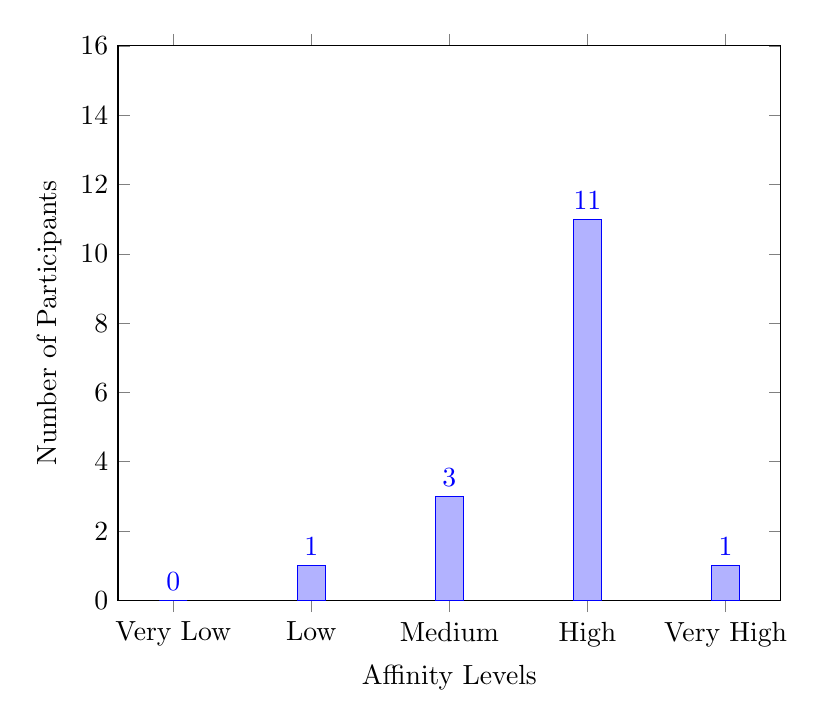
\begin{tikzpicture}
    \begin{axis}[
        ybar,
        symbolic x coords={Very Low, Low, Medium, High, Very High},
        xtick=data,
        nodes near coords,
        nodes near coords align={vertical},
        ymin=0,ymax=16,
        ylabel={Number of Participants},
        xlabel={Affinity Levels},
        %title={ATI-S Scale (Affinity for Technology Interaction)}
    ]
    \addplot coordinates {(Very Low,0) (Low,1) (Medium,3) (High,11) (Very High,1)};
    \end{axis}
\end{tikzpicture}
\caption{Distribution of Affinity for Technology Interaction among participants.}
\label{ati}
\end{figure}

A significant aspect of the participant profile is their technological affinity, as indicated by the Affinity for Technology Interaction Short Scale (ATI-S) values. This data revealed a pronounced tendency towards technology, with 12 participants scoring high or very high in technology affinity. This implies that the majority of participants were not only familiar with but also comfortable using technology, which is a crucial consideration in the context of phishing awareness and the effectiveness of warnings.

\section{Interview Results}

\textbf{Design Response}

Clarity and Legibility: Participants generally found the color red effective in drawing attention, with one noting \textit{"The red is just very catchy"} (P9), highlighting the visual impact of vibrant colors. The legibility of warnings was often a concern, as evidenced by comments such as \textit{"It’s the white on red what makes it difficult to read at times."} (P9), indicating difficulties with text contrast. 

Impact of Animations: Animations were noted for their effective attention-grabbing capabilities. For instance, one participant mentioned, \textit{"When the text field moves in like this, your eyes automatically move there."} (P2), showing how animations guide viewers' focus. A participant remarked on the possible negative impact of frequent animations, stating, \textit{"Moving warnings are more noticeable than ones that just appear on the screen. But if you put moving warnings on all phishing mails, it might be overwhelming and tire the eyes and mind. A balance is necessary. Maybe being too flashy, could even lead to desensitization over time."} (P5) Some participants also noted that the animations were too slow to appear, \textit{"It would be better if the warnings appeared immediately upon opening the email instead of having a delay"} (P5), which could lead to critical oversights. 
    
Placement: Participants commonly observed that warnings placed on the side of the email were less noticeable, often residing in their peripheral vision. As one participant expressed, \textit{"I actually found this one a bit inconspicuous because you have the email body here and the warning there. It reminds me of those advertisements on websites placed on the side of the page."} (P1) Conversely, warnings integrated directly into the email body proved to be more conspicuous. Participants reported that these warnings grabbed their attention immediately upon opening the email, as they were in the direct line of sight while reading the email content. 


\textbf{Perceived Helpfulness}

Context-Aware Warnings (Tooltip on Hover Over Link): This type of warning was generally seen as highly effective because it actively prevents clicks on potentially malicious links. A participant mentioned, \textit{"I believe the one covering the link was the most effective because it immediately prevented interaction."} (P6).
    
Content-Specific Warnings (Signature and Greeting Warnings): This type of warning was appreciated for its specificity, noting that these kind of details are easily overlooked in phishing emails: \textit{"I really liked the signature warnings. That could be something that might not catch the user’s attention at all."} (P5). A common point of criticism was, that this kind of warning is often not applicable, as not every email, especially in a non-business context, ends with a signature or uses a consistent greeting.
      
General Alerts: This type of warning received mixed feedback due to their positioning and the lack of detailed information they provided. Participants noted its visibility issues and expressed a preference for warnings that include explanatory details about the alert: \textit{"Those that just flew in and had standard text might be the weakest."} (P6). 

\textbf{Preferred Level of Detail}

A key theme that emerged from the interviews was a clear division in preference for either more detailed warnings or simpler alerts. Participants who favored more details appreciated the additional context and explanations provided in the warnings, which helped them understand why an email was flagged as suspicious. One participant stated, \textit{"I preferred the longer ones, because it teaches me how to recognize future phishing attempts."} (P11), emphasizing the educational aspect. Another point mentioned was the fact that a longer explanation might make it easier and more helpful for non tech-savy people. The Greeting Warning with interactive buttons presented a unique challenge during the study. While intended to enhance user engagement by providing direct context and proof, many participants either did not realize the buttons were clickable or hesitated to use them. This hesitation stemmed from a fear that interacting with the buttons might inadvertently lead them into a phishing trap. One participant expressed, \textit{"I wouldn’t like to click on those buttons if I would get such a warning. I don’t really know if I can trust it."} (P16). \par
Conversely, some participants (P5, P6) preferred simple warnings, valuing the straightforwardness and immediacy of the message without additional information. This preference indicates that for some users, efficiency and speed in email processing are prioritized over detailed educational content. 

\textbf{Novelties for Participants}

The qualitative data analysis underscored that many participants found the greeting and signature-specific warnings to be novel features. These aspects of the phishing warnings introduced new elements that participants had not previously encountered or considered significant in identifying phishing emails. As one participant reflected, \textit{"I have not seen such tailored warnings in phishing emails, which recognize a specific pattern and tell you why it's a phishing attempt. That is very new to me."} (P13). \newpage

\textbf{Refining Warning Design: Incorporating Feedback}

As outlined in section \ref{adjust}, modifications were made to the phishing warning designs beginning with participant 12. 
These changes were positively received, as indicated by subsequent participant feedback. Post-adjustment, there were no further complaints regarding the readability of the text or the timing of the animations, except for a single comment about the red tone being potentially too strong (P15). Participants appreciated the quicker responsiveness and greater clarity of the warnings, which effectively addressed the initial concerns raised about legibility and the timing of animation effects. 

\section{Eye Tracking Results}
\label{sec:eyetrackingres}
During the data analysis phase, it was noted that the eye tracking data for one participant (P14) was significantly lower in sample size compared to others. This anomaly could be attributed to improper seating position or a flawed calibration process. To maintain the integrity and reliability of the analysis, this participant's data was excluded, resulting in a total of 15 eye tracking samples being considered for the final evaluation.

A full export of our raw eyetracking data is provided in the GitHub repository linked in appendix \ref{sec:github}.


\textbf{H1: Delayed Animation's Influence on Reading Pattern}

Eye tracking data indicated no significant disruption in reading patterns due to delayed animations in phishing warnings. Observing the gaze patterns showed that the onset timing of animations, whether immediate or delayed, did not alter the attention flow significantly. Users exhibited similar engagement with immediate and delayed warning presentations, suggesting a uniform approach to processing these visual cues.

\textbf{H2: Visibility of Side-Placed Warnings} 

The eye tracking analysis showed that warnings positioned on the side of the email interface captured attention quickly but consistently later than other warnings. The focus of gaze primarily remained on the other areas of the emails, with peripheral warnings drawing attention only after the central and top content had been reviewed. This observation was consistent across the study's participants, supporting the hypothesis that side-placed warnings are less immediately noticeable. \newline Eye tracking data (figure \ref{sideaoi}) supports this finding, showing that the median time taken for participants to first fixate on the Side AOI was approximately 2 seconds. To put this in contrast we compared this to the Top AOI data, where we recorded a notably quicker median time to first fixation of approximately 1.2 seconds.  

\textbf{H3: Sustained Engagement of Body-Integrated Warnings}

Data strongly supported the hypothesis that warnings integrated directly into the email body were engaged with more thoroughly by users than those placed at the side. The analysis of average fixation durations (figure \ref{avgfix}) revealed that engagement times for the Center AOI were generally longer across participants. However, there were notable exceptions for participants 7 and 13, where the fixation duration on the Center AOI was shorter compared to the other participants. 

\begin{figure}[H]
\centering
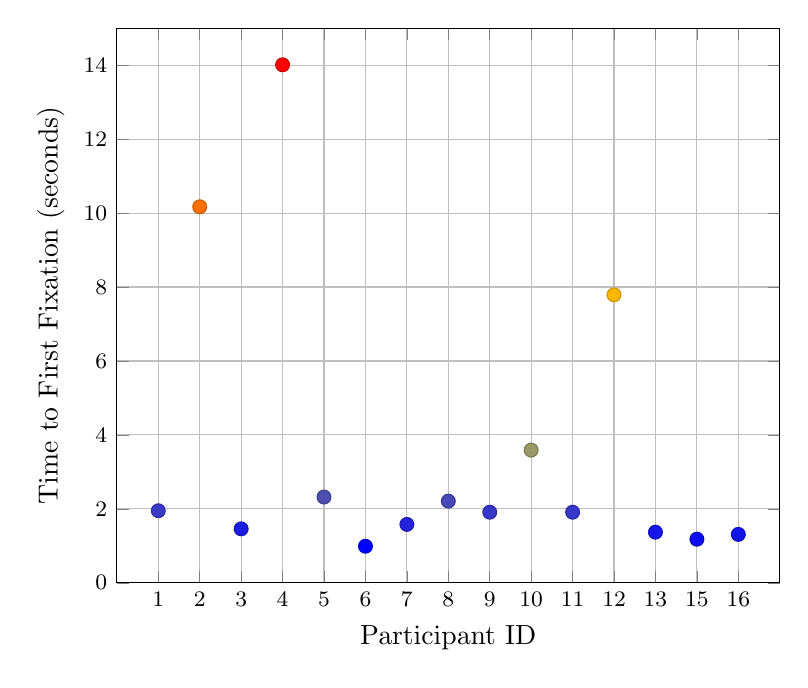
\begin{tikzpicture}
\begin{axis}[
    xlabel={Participant ID},
    ylabel={Time to First Fixation (seconds)},
    grid=major,
    xmin=0, xmax=16, 
    ymin=0, ymax=15,  
    xtick={1,2,...,15}, 
    xticklabels={1,2,...,12,13,15,16}, 
    xticklabel style={font=\footnotesize, rotate=0}, 
    yticklabel style={font=\footnotesize}
]
\addplot+[
    only marks,
    mark=*,
    mark size=2.5pt,
    scatter=true, 
    color=blue, 
    fill=blue  
] table [row sep=\\,y=data, x=seq] {
    seq  data\\
    1    1.95\\ 2    10.17\\ 3    1.46\\ 4    14.01\\ 5    2.32\\
    6    0.99\\ 7    1.58\\ 8    2.21\\ 9    1.91\\ 10   3.59\\
    11   1.91\\ 12   7.79\\ 13   1.37\\ 14   1.18\\ 15   1.31\\
};
\end{axis}
\end{tikzpicture}
\caption{Time to first fixation for the side AOI.}
\label{sideaoi}
\end{figure}

\begin{figure}[H]
\centering
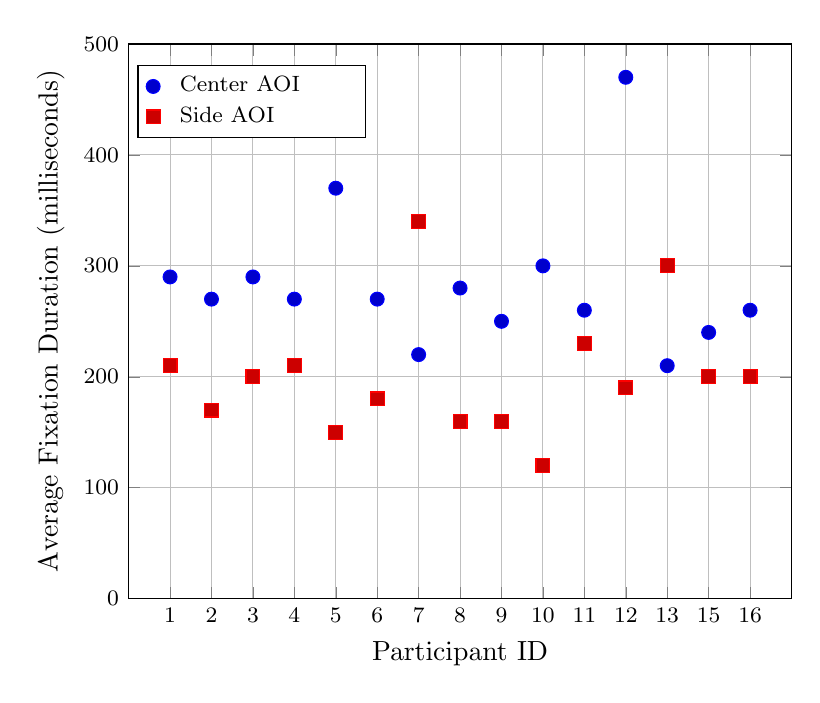
\begin{tikzpicture}
\begin{axis}[
    xlabel={Participant ID},
    ylabel={Average Fixation Duration (milliseconds)},
    grid=major,
    xmin=0, xmax=16, 
    ymin=0, ymax=500,
    xtick={1,2,...,15}, 
    xticklabels={1,2,...,12,13,15,16}, 
    ytick={0, 100,200,300,400,500}, 
    xticklabel style={font=\footnotesize}, 
    yticklabel style={font=\footnotesize},
    legend style={
        at={(0.1855,0.83)},
        anchor=south,
        text width=2cm, 
        minimum width=2.5cm, 
        font=\footnotesize 
    }
]
\addplot+[
    scatter,
    only marks,
    mark=*,
    mark size=2.5pt,
    scatter=false,
    color=blue, 
    fill=blue 
] coordinates {
    (1,290) (2,270) (3,290) (4,270) (5,370)
    (6,270) (7,220) (8,280) (9,250) (10,300)
    (11,260) (12,470) (13,210) (14,240) (15,260)
};
\addplot+[
    scatter,
    only marks,
    mark=square*,
    mark size=2.5pt,
    scatter=false,
    color=red, 
    fill=red
] coordinates {
    (1,210) (2,170) (3,200) (4,210) (5,150)
    (6,180) (7,340) (8,160) (9,160) (10,120)
    (11,230) (12,190) (13,300) (14,200) (15,200)
};
\legend{Center AOI,Side AOI}
\end{axis}
\end{tikzpicture}
\caption{Comparison of the average fixation duration for center and side AOIs.}
\label{avgfix}
\end{figure}

\chapter{Discussion}
\section{Interpretation of Qualitative Feedback}
\subsection{Emerging Themes and Best Practices}
The qualitative feedback analysis illuminates several emerging themes that contribute to the effectiveness of phishing warnings. Reflecting on these, we can delineate best practices for designing phishing warning systems that align with user expectations.

\textbf{Attention-Grabbing without being Overwhelming}

A recurring theme is the delicate balance between capturing users’ attention and avoiding sensory overload. Warnings that are too subtle may go unnoticed, while those that are too aggressive could be dismissed as annoyances. Best practices suggest employing moderate animations and placing warnings within the users' immediate visual field. For example, one participant noted, \textit{"When the text field moves in like this, your eyes automatically move there."} (P2) indicating the value of animated cues. However, animations should not be excessively flashy or complex, as they risk desensitizing users over time. Supporting this, a study on the effects of animation in online contexts found that while animations increase visibility and engagement, they must be balanced to avoid overshadowing important content or overwhelming the viewer \cite{cheung}.

\textbf{Clarity and Contextual Information}

Clarity in warning messages is essential. Participants expressed a preference for warnings with a clear and legible typography set against a contrasting background, improving readability. The use of the color red was frequently mentioned as effective due to its association with caution and urgency. \newline 
Moreover, providing contextual information within the warning, such as the reason an email was flagged and highlighting subtle language cues, such as the greeting, can enhance users’ understanding and prompt more informed action. As one user aptly put it, \textit{"I preferred the longer ones, because it teaches me how to recognize phishing attempts."} (P11), highlighting the educative function. \newline
This emphasis on context-rich warnings aligns with findings from other studies \cite{buono, aneke}, which also highlight the importance of explanatory warnings in phishing emails, thus not only alerting users to immediate threats but also equipping them with knowledge that could prevent future phishing attacks. Such strategies are crucial for improving user understanding and ensuring that warnings lead to informed actions and thereby enhancing the overall effectiveness of phishing warnings.

\textbf{Trust and Interactivity}

The trustworthiness of warnings is key; users must feel confident interacting with them. This includes a hesitance to engage with clickable elements within the warnings due to fear of intensifying a potential threat. Best practices would therefore involve clearly distinguishing warning elements from potential phishing mechanisms and ensuring that interactive components, when used, are immediately recognizable as safe and official parts of the email client interface.

\textbf{Incorporating User Feedback for Iterative Improvement}

The inclusion of user feedback into the design process is not only beneficial but essential for the development of effective phishing warnings. Adjustments made in response to participant insights, such as enhancing color contrast to improve legibility, exemplify how iterative design based on user experience can significantly help in designing effective security measures. As highlighted in the article by Grobler et al. \cite{grobler} actively engaging users in refining security solutions helps tailor these systems to better meet their needs and expectations, thereby increasing their efficacy and user adoption rates. Best practices would therefore advocate for continuous user testing and refinement, ensuring that warnings adapt over time to align with evolving user behaviors and phishing tactics. This proactive approach ensures that security measures remain robust, user-friendly, and effective in real-world scenarios.

\subsection{Summary: Users’ Perceptions of Phishing Warnings}
To address RQ1 regarding user perceptions and the effectiveness of various phishing warnings in email interfaces, we analyzed qualitative feedback from participants. The effectiveness was assessed based on the ability of warnings to enhance user awareness, encourage appropriate actions to mitigate risks, such as not clicking on malicious links, and improve recognition of phishing threats in future encounters.

\textbf{Perceived Helpfulness and Effectiveness of Warning Types}
\begin{enumerate}
    \item \textbf{Context-Aware Warnings (Tooltip on Hover Over Link):}
    Participants found context-aware warnings extremely effective. These warnings prevent direct interaction with malicious links, thereby immediately mitigating risk. This direct intervention makes them highly valuable in protecting users in real-time.
    \item \textbf{Content-Specific Warnings (Signature and Greeting Warnings):}
    These warnings are appreciated for their specificity and relevance, particularly in environments where consistency is expected, such as professional emails. They provide clear and relevant context by highlighting anomalies in expected email patterns, offering a direct comparison with typical content. Their educational value is significant as they enhance users' ability to identify subtle signs of phishing attempts, which might otherwise be overlooked.
    \item \textbf{Generic Banners:}
    Generic banners received the least favorable feedback. Their effectiveness was often questioned due to poor placement and lack of detailed information, which led to them being easily ignored. Especially variant 2 (side placed banner) was criticized for being too inconsipicous. Participants compared its noticeability to peripheral advertisements on websites, which are often disregarded due to desensitization. This feedback highlights the importance of not only the placement of warning banners but also the inclusion of specific reasons why an email might be flagged as potentially dangerous, enhancing user understanding and response to phishing threats.
\end{enumerate}

\textbf{Preferred Warning Design}

From the feedback, it's clear that users prefer warnings that are not only visible but also informative. Warnings that blend seamlessly into the user's workflow in the email interface, such as those integrated within the primary content, are particularly effective. These warnings grab attention quickly, provide essential information, and are directly interacted with, enhancing both immediate and long-term phishing threat recognition.

\definecolor{Ebb}{rgb}{0.925,0.894,0.894}
\begin{table} [H]
\centering
\begin{tblr}{
  row{1} = {Ebb},
  hlines,
  vlines,
  hline{1,5} = {-}{0.08em},
  colspec = {X[1.75,l] X[2.25,l] X[4,l]},
}
\textbf{Warning Type}     & \textbf{Key Feature}                 & \textbf{User Feedback}                                                                                                      \\
Context-Aware       & Actively prevents clicking on links  & Very positive; users felt it was very effective and helpful, appreciating the proactive nature of the warning.              \\
Content-Specific    & Highlights anomalies in the language & Positive; users appreciated their specificity and educational value, noting they felt more informed about phishing tactics. \\
General             & Broad, non-specific warning          & Less favorable; often overlooked, reported by users as too generic and lacking actionable details.                          
\end{tblr}
\caption{Overview of warning types and user feedback.}
\label{tab:types}
\end{table}

\section{Interpretation of Eye Tracking Results}

\subsection{Impact of Delayed Animations}

Our hypothesis that delayed animations would disrupt the typical email reading pattern and draw more attention was not supported by the data. The implications suggest that while animations serve as useful attention-grabbing tools, their effectiveness does not necessarily benefit from a delayed presentation. Aligning with the qualitative interview results, it appears that ensuring the visibility of warnings immediately upon email viewing is more crucial for capturing attention and facilitating prompt user reactions. \newline
However, it is important to note, that the evaluation of this hypothesis may be limited by the methodology used. Only 4 participants tested the new warnings with no animation delay, which may not provide a sufficiently robust dataset to draw definitive conclusions.

\subsection{Effective Warning Placement}

The data supports that warnings placed within the central viewing area of an email are engaged with more extensively. This is evidenced by generally longer average fixation durations on the Center AOI. These findings underscore the efficacy of aligning warning placements with natural reading behaviors, thereby enhancing the visibility and impact of security warnings. \newline However, the analysis revealed notable deviations for participants 7 and 13, who exhibited shorter fixation durations on the Center AOI compared to other participants. This variability in user interaction suggests that while centrally-placed warnings are generally effective, their impact can vary significantly among users due to individual differences in reading habits or the visual salience of the warnings. \newline
The extended engagement with central warnings highlights their effectiveness in maintaining user attention, which is crucial for ensuring that warnings are not only noticed but also sufficiently processed. This is vital for the effective communication of security-related information. Based on these insights, designers are encouraged to position crucial information and alerts within the central visual field to maximize their impact. Furthermore, understanding the reasons behind the shorter fixation times for specific participants could inform more tailored design approaches, ensuring that warnings are effective across a diverse user base.

In contrast, warnings positioned on the periphery of the email interface, such as on the sides, were consistently noticed later and engaged with less extensively. Although our data indicates only a slight delay in detection, this brief period can be critical, particularly during a hectic workday when users may be under pressure or multitasking. This oversight provides a window during which users could inadvertently interact with deceptive links or other malicious content. Moreover, the presence of outliers where the time to first fixation was exceedingly long highlights the potential severity of this issue. \newline
Furthermore, the average fixation duration on these side-placed warnings was also notably lower than that for central warnings, suggesting that even when the warning is noticed, the engagement is less intensive. This lack of deep engagement suggests that the warnings may not be registering effectively with users. This observation aligns with participant feedback, where many reported not noticing the side-placed warnings at all, despite eye tracking data confirming visual detection. \newline
This phenomenon, supported by the comments of two participants (P1, P9), reinforces the argument that peripheral warnings may be less effective due to a learned tendency to disregard non-central elements. The reduced fixation durations further signify that users engage only superficially with these warnings when they do notice them, which could seriously undermine their effectiveness in security-sensitive environments.

\subsection{Summary: Gaze Patterns and Warning Placement}

RQ2 explores how common gaze patterns among users can inform the strategic placement of phishing warnings. The analysis confirms a predominant focus on the central area of the email interface, a natural result of typical reading behaviors. This focal tendency significantly benefits the placement of warnings directly within this central area, ensuring they are both quickly noticed and more actively engaged with.

These insights provide a robust foundation for future email interface designs, suggesting that to maximize the impact of phishing warnings, designers should prioritize central visual placement of critical security cues. This approach will significantly improve defense mechanisms against phishing attacks, ensuring that warnings are not only visible but also integrated into the flow of natural user interactions with email content.

\section{Limitations}

\subsection{Participant Diversity and Sample Size}
The majority of our participants were drawn from a similar demographic group, predominantly consisting of university students and young adults within the same age range and academic environment. Moreover, a significant portion of participants demonstrated a high Affinity for Technological Interaction (ATI), as illustrated in figure \ref{ati}. This heightened technological comfort and skill among our sample may not accurately represent the broader population's varying levels of technological proficiency. The lack of diversity in our sample, both demographically and in terms of technological affinity, could limit the generalizability of our findings across a broader population and potentially introduce biases in the evaluation of our phishing warnings. For example, older adults might interpret and respond to visual cues differently due to variations in technological fluency and cognitive processing speeds, which may differ markedly from the responses observed in younger, more technologically adept participants \cite{age}. \newline
Additionally, the iterative design adjustment made based on participant feedback later in the study highlighted another significant limitation related to sample size. After implementing changes to the warning designs, it was planned to test these modifications with eight additional participants. Unfortunately, only four additional participants were able to participate in the study. This smaller-than-expected sample size of participants might not provide a sufficiently robust dataset to draw definitive conclusions about the effectiveness of the redesigned warnings.

\subsection{Alert Fatigue}
An important aspect, which we did not explore in this study, is the potential for alert fatigue, a phenomenon where users become desensitized to warnings due to frequent exposure. This desensitization can result in reduced effectiveness of the warnings over time \cite{ban}. \newline While our study focused on the immediate effectiveness of different phishing warning designs, it did not account for the long-term impact of repeated exposure to these warnings. To mitigate the effects of alert fatigue, future research could explore strategies such as varying the design and presentation of warnings. Additionally, longitudinal studies could assess the impact of repeated exposure to phishing warnings over an extended period and provide valuable insights into how to design more resilient warning systems.

\subsection{Study Setup and Ecological Validity}
The use of a controlled lab environment to conduct this study poses significant limitations regarding ecological validity. Participants were aware that their actions were being observed, potentially influencing their behavior—a phenomenon known as the Hawthorne effect \cite{jim}. This awareness can alter natural responses and may not accurately reflect their behavior in less controlled environments. \newline
Furthermore, the artificial nature of the study environment can significantly impact participants' risk perception \cite{garfinkel}. Since the risk to personal data is non-existent in a simulated phishing attack, participants' reactions to warnings and their decision-making processes might not truly reflect their actions in a real threat scenario. This discrepancy can skew results related to actual risk perceptions and behaviors, potentially leading to overestimations of the effectiveness of warning systems in genuine contexts.

\chapter{Conclusion}
\label{sec:conclusion}
This thesis has extensively investigated the impact of various visual warning designs on user responses to phishing threats in email clients. The use of eye tracking technology and qualitative feedback has provided a deep understanding of how different warning strategies affect user behaviour and engagement.

The research conclusively demonstrates that integrating warnings directly within the email content markedly enhances both the immediacy of user reactions and their overall engagement with the warnings. These findings underline the importance of prominent, context-rich warnings that are easily visible and provide actionable information to users.

Furthermore, the study highlights the crucial role of educational content in warnings. Clear, informative warnings not only alert users to immediate threats but also educate them, enhancing their ability to identify similar threats independently in the future. This dual function of warnings is vital in the ongoing battle against phishing, as well-informed users are the first line of defense in cybersecurity.

However, the study also highlights significant opportunities for expansion in both scope and realism for future research. A crucial first step is broadening the participant pool to include a more diverse range of ages, professions, educational backgrounds, and increasing sample sizes to ensure findings are robust and generalizable. This will enhance our understanding of how different user groups perceive and react to phishing threats, supporting the development of more universally effective defensive measures. Additionally, to significantly boost ecological validity, future studies could integrate phishing detection research into real-world user environments. This advancement might entail the development and application of phishing detection algorithms capable of operating effectively within users' naturalistic settings. Such a move would not only provide more authentic data but also allow for a robust assessment of phishing warning effectiveness under typical usage conditions.

Looking forward, the rapid advancement of artificial intelligence and large language models opens new frontiers for phishing defense. These technologies could be leveraged to develop more adaptive, personalized phishing detection and prevention strategies, enhancing the precision and responsiveness of warnings. For instance, AI could analyze user behavior to tailor warnings to individual risk profiles or detect subtle phishing attempts that evade traditional detection methods. This proactive and technologically innovative approach is crucial in an era where cyber threats are continually evolving, thus ensuring the digital safety of users globally. As cybercriminals become more sophisticated, integrating cutting-edge technologies into cybersecurity measures will be essential for staying ahead of threats and safeguarding digital interactions.

%%%%%%%%%%%%%%%%%%%%%%%%%%%%%%%%%%%%%%%%%%%%%%%%%%%%%%%%%%%%%%%%%%%%%%%%%%%%%%
%
% Main content ends here
%
%%%%%%%%%%%%%%%%%%%%%%%%%%%%%%%%%%%%%%%%%%%%%%%%%%%%%%%%%%%%%%%%%%%%%%%%%%%%%%


\printbibliography

All links were last followed on \today{}.

\appendix
\chapter{Appendix}

\section{GitHub Repository}
\label{sec:github}

{\large \faGithub} \hspace{2pt} \href{https://github.com/yunuseyvz/Bachelorthesis_Phishing}{github.com/yunuseyvz/Bachelorthesis\_Phishing}

\par
This public repository contains: 

\begin{itemize}
    \item Email Samples
    \item Thunderbird Plugin Sourcecode
    \item Python Script Sourcecode
    \item Eyetracking Data Exports 
    \item MAXQDA2024 Project Files 
    \item Transcripts (\textit{Note: Transcripts have been manually reviewed. Irrelevant and personal information have been removed.})

\end{itemize}

\section{Study Protocol}
\label{sec:protocol}

\textbf{Pre-Setup}
\begin{itemize}
    \item Software Setup: Set up Mozilla Thunderbird on the participant's computer, installing the necessary addon that will be used during the study. Ensure that all settings are optimal for the tasks ahead. Install Tobii Pro Lab for extensive eye tracking tools.
    \item Seating Arrangement: Arrange for a non-rolling chair to minimize movement and ensure more accurate eye tracking data.
    \item Eye Tracker: Attach and setup the eye tracker.
    \item Moderator's Setup (optional): Arrange a second screen for the moderator in Tobii Pro Lab to monitor and observe the eye tracking data in real-time.
\end{itemize}

\textbf{Welcome and Consent}
\begin{itemize}
    \item Introduction to the Study: 
    \begin{itemize}
        \item[ ]\textit{"Hello and welcome! Thank you for participating in our study today.  I will be guiding you through the process and the session will last about 30 minutes. You will get a small task where you need to sort through a fictional inbox, I will explain in detail when we get there. While doing that we will have an eye tracker running, which will track and record you eye movements. After the sorting task I will ask you a couple of questions."}
    \end{itemize}
\newpage
    \item Consent Form:
        \begin{itemize}
            \item[ ]\textit{ "Before we begin, please take a moment to read this consent form. If everything is clear, please sign the form at the bottom."}
        \end{itemize}
        
\end{itemize}

\textbf{Before Beginning}
\begin{itemize}
    \item Eye Tracker Calibration and Audio Recording
        \begin{itemize}
            \item[] \textit{"Our first step will be to calibrate the eye tracker for a more accurate data capture. Just follow the instructions on the screen. This will take around 30 seconds. (...) "Thank you for that. Now we can begin with the task. I will also start the audio recording now."}
        \end{itemize}
\end{itemize}

\textbf{Phase 1: Email Sorting (Approximately 10 Minutes)}
\begin{itemize}
    \item Task Description:
        \begin{itemize}
            \item[] \textit{"In this part, you will act as an employee at 'Cloudtech'. Your task is to sort through your emails as you would in your work inbox. You only need to decide whether to delete each email or keep it. No other actions are necessary. "As you sort through the emails, please try to verbalize your thoughts. Say out loud what you are thinking about each decision. This helps us understand your reasoning. Feel free to open any links or attachments in the emails as you see fit. Interact with the emails as you would normally. Let me know when you are done."}
        \end{itemize}
    \item Task Finished:
        \begin{itemize}
            \item[] \textit{"Alright, thank you. Now we will get to the second phase of the study."}
        \end{itemize}
\end{itemize}

\textbf{Part 2: Detailed Interview (Approximately 10 Minutes)}
\begin{itemize}
    \item Debriefing:
        \begin{itemize}
            \item[] \textit{"Before we move on to the interview I will debrief you on what this study is about. Our study is about how users interact and engage with different types of visual warnings in email clients. For that we first collect eyetracking data for an objective view. After that we conduct a small semi-structured interview to ask you about your subjective experiences with the warnings. Before we move on, I will briefly show you through the warnings again. (...) Alright now to the questions."}
        \end{itemize}
    \item Interview: 
        \begin{itemize}
            \item[] \textit{See appendix \ref{sec:interview}.}
        \end{itemize}
    
\end{itemize}

\textbf{Conclusion of the Session}
\begin{itemize}
    \item Compensation: 
        \begin{itemize}
            \item[] \textit{"Alright. Thanks a lot for participating! You will be compensated with 10€ via PayPal or bank transfer. I will send you a link, where you can enter your payment information. Alternatively you can opt for 1 MMI point, if you are a Media Informatics Student."}
        \end{itemize}
    \item Thank You and Farewell: 
        \begin{itemize}
            \item[] \textit{"Your input is very valuable to our research. Thank you again for your time today. Have a great day!"}
        \end{itemize}
\end{itemize}

\section{Interview Questions}
\label{sec:interview}
These are the questions posed to the participants in the second phase. Note that the interview was semi-structured so deviations and follow up questions were possible.

\textbf{General Perception:}

\begin{itemize}
    \item How did you generally perceive the warnings? Did they immediately stand out?
    \item Follow-up questions, e.g., if "Good", ask why exactly good or bad.
    \item Were there elements in the warnings that particularly stood out to you? What caught your attention the most?
    \item What role did the warning notices play in your decisions?
\end{itemize}

\textbf{Effectiveness of the Warnings:
}
    \begin{itemize}
        \item How do you assess the effectiveness of the various warning notices presented to you during the study?
        \item Were there any warning notices you found particularly helpful or less helpful?
        \item Each warning notice had 2 versions (simple/detailed). Which version do you prefer, and why? (Show the warnings again)
    \end{itemize}

\textbf{Design of the Warning Notices:}

    \begin{itemize}
        \item How do you evaluate the design of the warning notices (e.g., color, placement, animations)? Did these influence your attention?
        \item How do you assess interactive elements in warning notices (e.g., greeting warning)?
        \item Do you have any suggestions for improving the design of the warning notices?
    \end{itemize}

\textbf{Personal Behavior:
}
    \begin{itemize}
        \item Were there any pieces of information in the warnings that you hadn't paid attention to before?
        \item How do you usually handle emails once there's a suspicion of phishing? Or what specifically do you look at once there's a suspicion?
    \end{itemize}

\textbf{Feedback:
}
    \begin{itemize}
        \item Do you have any suggestions on how we could improve the study in the future?
        \item Do you have any other questions or comments?
    \end{itemize}

\newpage   
\section{Warning Designs}
\label{sec:warnings}
Below is an overview of version 1 of each warning type.
\par
\par
\begin{figure} [H]
\centering
\begin{subfigure}{.5\textwidth}
  \centering
  \includegraphics[width=1\linewidth]{figures/banner1_old.png}
  \caption{Variant 1}
\end{subfigure}%
\begin{subfigure}{.5\textwidth}
  \centering
  \includegraphics[width=1\linewidth]{figures/banner2_old.png}
  \caption{Variant 2}
\end{subfigure}
\caption{Generic Banner (Version 1)}
\end{figure}

\begin{figure} [H]
\centering
\begin{subfigure}{.5\textwidth}
  \centering
  \includegraphics[width=1\linewidth]{figures/hover1_old.png}
  \caption{Variant 1}
\end{subfigure}%
\begin{subfigure}{.5\textwidth}
  \centering
  \includegraphics[width=1\linewidth]{figures/hover2_old.png}
  \caption{Variant 2}
\end{subfigure}
\caption{Tooltip Warning on Link Hover (Version 1)}
\end{figure}

\begin{figure} [H]
\centering
\begin{subfigure}{.5\textwidth}
  \centering
  \includegraphics[width=1\linewidth]{figures/sig1_old.png}
  \caption{Variant 1}
\end{subfigure}%
\begin{subfigure}{.5\textwidth}
  \centering
  \includegraphics[width=1\linewidth]{figures/sig2_old.png}
  \caption{Variant 2}
\end{subfigure}
\caption{Signature-Specific Warning (Version 1)}
\end{figure}

\begin{figure} [H]
\centering
\begin{subfigure}{.5\textwidth}
  \centering
  \includegraphics[width=1\linewidth]{figures/greeting1_old.png}
  \caption{Variant 1}
\end{subfigure}%
\begin{subfigure}{.5\textwidth}
  \centering
  \includegraphics[width=1\linewidth]{figures/greeting2_old.png}
  \caption{Variant 2}
\end{subfigure}
\caption{Greeting-Specific Warning (Version 1)}
\end{figure}

\newpage
\section{QDA Codebook}
\label{sec:qda}
Below is the list of codes developed and utilized during the qualitative data analysis process of our study.
\begin{itemize}
    \item Design Response: This code looks into the overall aesthetic and functional reception of the warning designs by the participants.
    \begin{itemize}
        \item Clarity and Legibility: Evaluates how easily the warnings can be read and understood.
        \item Impact of Animations: Assesses how motion and dynamic elements in the warnings affect user attention and understanding.
        \item Placement: Considers the effectiveness of where warnings are located within the email interface.
        \item Potential Improvements: Gathers participant suggestions on how to enhance the warning designs.
        \item User Attention: Analyzes how conspicuous or inconspicuous these warnings are to the users.
        \begin{itemize}
            \item Conspicuous: Warnings that are immediately noticeable.
            \item  Inconspicuous: Warnings that tend to be overlooked.
        \end{itemize}
    \end{itemize}
    \item Novelties for Participants: Identifies aspects of the phishing warnings that were particularly novel or unexpected to the participants.
    \item Perceived Helpfulness: Explores participants' perception on each warnings helpfulness.
    \begin{itemize}
        \item Negative: Participant feedback that highlights shortcomings or ineffective aspects of the warnings.
        \item Positive: Positive reactions that underscore the effectiveness and utility of the warnings.
        \item Prefered Complexity: Explores participants' preferences for the complexity of the information provided in the warnings.
        \begin{itemize}
            \item More Details: Preference for detailed and informative warnings.
            \item Simplicity: Preference for straightforward, minimal warnings.
        \end{itemize}
    \end{itemize}
\end{itemize}

\newpage
\section{Eye Tracking Heatmap}

\iffalse
\begin{figure}[H]
\centering
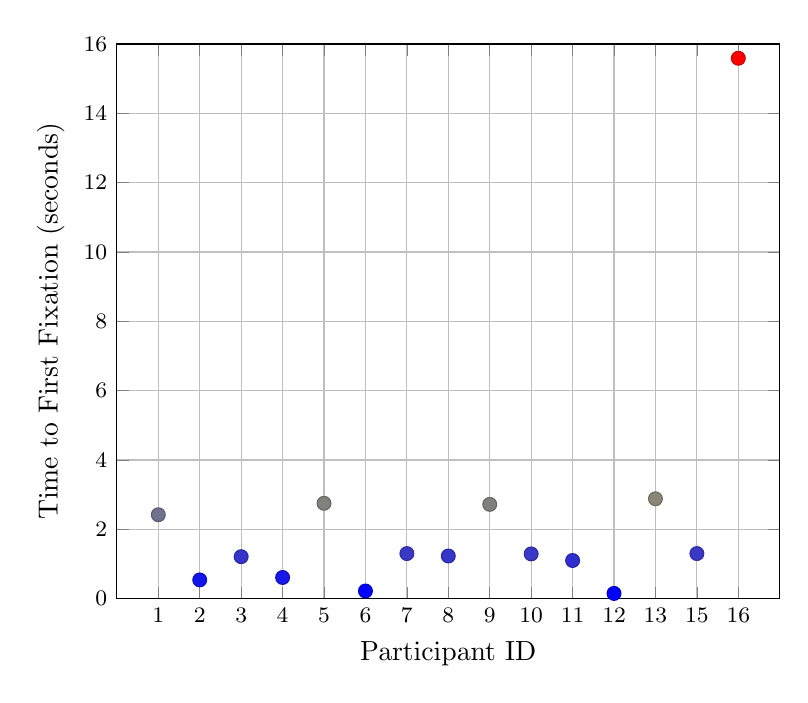
\begin{tikzpicture}
\begin{axis}[
    xlabel={Participant ID},
    ylabel={Time to First Fixation (seconds)},
    grid=major,
    xmin=0, xmax=16, 
    ymin=0, ymax=16,  
    xtick={1,2,...,15}, 
    xticklabels={1,2,...,12,13,15,16}, 
    xticklabel style={font=\footnotesize, rotate=0}, 
    yticklabel style={font=\footnotesize}
]
\addplot+[
    only marks,
    mark=*,
    mark size=2.5pt,
    scatter=true, 
    color=blue, 
    fill=blue  
] table [row sep=\\,y=data, x=seq] {
    seq  data\\
    1    2.42\\ 2    0.54\\ 3    1.21\\ 4    0.61\\ 5    2.75\\
    6    0.22\\ 7    1.30\\ 8    1.23\\ 9    2.72\\ 10   1.29\\
    11   1.10\\ 12   0.15\\ 13   2.88\\ 14   1.30\\ 15   15.59\\
};
\end{axis}
\end{tikzpicture}
\caption{Time to first fixation for the top AOI.}
\label{sideaoi}
\end{figure}
\fi

Included here is an eye tracking heatmap using the gaze data of all participants. Although not directly referenced in the main findings, this heatmap may serve as a useful resource for other researchers interested in the visual patterns of user interaction. It also serves an educational purpose, illustrating the application of eye tracking technology in research.

\begin{figure} [ht]
    \centering
    \includegraphics[width=1\linewidth]{figures/heatmap_overlay.png}
    \caption{Accumulated eyetracking heatmap, generated in Tobii Pro Lab}
    \label{fig:heatmap}
\end{figure}

%\input{latexhints/latexhints-english}

\pagestyle{empty}
\renewcommand*{\chapterpagestyle}{empty}
\Affirmation
\end{document}
